
\documentclass[man, 12pt, a4paper]{apa7}
%\usepackage{geometry}
% \geometry{
% a4paper,
% marginparwidth=30mm,
% right=40mm,
% }

\usepackage[american]{babel}
\usepackage[utf8]{inputenc}
\usepackage{csquotes}
\usepackage{hyperref}
\usepackage[style=apa,sortcites=true,sorting=nyt, backend=biber, natbib=true, uniquename=false, uniquelist=false, useprefix=true]{biblatex}
\usepackage{authblk}
\usepackage{amsmath}
\usepackage{graphicx}
\usepackage{setspace,caption}
\usepackage{subcaption}
\usepackage{enumitem}
\usepackage{lipsum}
\usepackage{xcolor}
\usepackage{fourier}
\usepackage{stackengine}
\usepackage{scalerel}
\usepackage{fontawesome}
\usepackage[normalem]{ulem}
\usepackage{longtable}

% Select what to do with todonotes: 
% \usepackage[disable]{todonotes} % notes not showed
\usepackage[draft]{todonotes}   % notes showed

% Select what to do with command \comment:  
% \newcommand{\comment}[1]{}  %comment not showed
\newcommand{\comment}[1]
{\par {\bfseries \color{blue} #1 \par}} %comment showed

% make warning with red triangle
\newcommand\Warning[1][2ex]{%
  \renewcommand\stacktype{L}%
  \scaleto{\stackon[1.3pt]{\color{red}$\triangle$}{\tiny\bfseries !}}{#1}}%


\hypersetup{
pdfpagemode={UseOutlines},
bookmarksopen=true,
bookmarksopenlevel=0,
hypertexnames=false,
colorlinks   = true, %Colours links instead of ugly boxes
urlcolor     = blue, %Colour for external hyperlinks
linkcolor    = blue, %Colour of internal links
citecolor   = cyan, %Colour of citations
pdfstartview={FitV},
unicode,
breaklinks=true,
}

\DeclareLanguageMapping{american}{american-apa}
\addbibresource{references.bib}

\title{Integration of Migrants: A Systematic Review, Descriptive Conceptual Framework, (and Meta-Analysis?)}
\shorttitle{Integration of Migrants}

\author[*,1,2]{Jannis Kreienkamp}
\author[1,2]{Kai Epstude}
\author[1,2]{Laura F. Bringmann}
\author[1,2]{Peter de Jonge}
\affiliation{\hfill}
\affil[1]{University of Groningen, Department of Psychology}
\affil[2]{Author order still to be decided (sorted alphabetically by first name)}

\authornote{
   \addORCIDlink{* Jannis Kreienkamp}{0000-0002-1831-5604}

We have no known conflict of interest to declare.

Correspondence concerning this article should be addressed to Jannis Kreienkamp, Department of Psychology, University of Groningen, Grote Kruisstraat 2/1, 9712 TS Groningen (The Netherlands).  E-mail: j.kreienkamp@rug.nl}

\leftheader{Kreienkamp}

\abstract{Abstract goes here.}

\keywords{Keyword \#1, Keyword \#2, ...}

\setlength\parindent{1.27cm}

\begin{document}
\maketitle

\todo[inline]{*Relevance*} 
The adaptation of migrants in new cultural contexts is an important issue in many societies around the world. With many of the migration push and pull factors in the economic, safety, social, and environmental domains worsening, the topic is likely to become even more important in the future (Reference).
% Possible examples: violence and abuse of power (e.g., war, persecution; asylum seekers and refugees), social and economic disparities increasing (e.g., education, services, career; migrant workers, labor migrants), disproportionate environmental injustice (e.g., natural disasters, pollution, crop failure; environmental migrants). Together with population growth and globalisation.
The current challenges and increasing migration highlight once more how important it is to understand how adaptation processes unfold and which aspects are most important to positive and sustainable outcomes. 

\todo[inline]{*Problem*} 
One of the fundamental challenges to psychological integration, faced by researchers, practitioners, and policy-makers, is an essentially scattered field with immense heterogeneity in definitions and measures of individual cultural adaptation\footnote{\textbf{I know this is way too long and we should probably just use `acculturation' and make a note that we mean the original meaning.} Researchers have used a wide range of terms in the context of cultural interactions, including acculturation, enculturation, transculturation, assimilation, integration, and cultural adaptation, -adjustment, or -transition. While there are often important conceptual differences between the terms, they all aim to capture and describe a process of change when two cultures interact. In this paper we will mostly use the term \textit{cultural adaptation}. The term `adaptation' in its etymology takes a functional approach -- where both individuals and interactive systems adjust to be better suited for their environment. In this understanding, cultural adaptation is (1) relevant on an individual- as well as on a group level, (2) places responsibility on any individual and group in the environment, and (3) is inherently a temporal and interactive process. Note that we do not specify what exactly is adaptive in any circumstance and that 'adaptation' is not a necessary outcome (i.e., many change processes do not enhance the livability of groups or individuals). Cultural adaptation rather seems to be a target that underlies most measures and definitions in the field -- even if only for one of the interacting groups. We also want to highlight that the term (psychological) acculturation was originally referred to as a neutral and descriptive umbrella term, which shares many of these attributes (e.g., \citealp{Berry2003}). Yet, we chose not to use acculturation as our primary term because over the past 90 years users of the term have most frequently used it in a static manner \citep{Brown2011, Ward2019} and have placed disproportional responsibility on migrants \citep{Bourhis1997a} -- despite its more neutral original intention \citep[e.g.,][]{Berry2009a}. We believe that part of this confusion stems from the word itself, where the ac- prefix indicates a movement (of an individual) towards a cultured end-state. Yet, because the term \textit{acculturation} is often used in the psychological literature and the term \textit{integration} is widely used in societal debates, we will, at times, use these terms interchangeably.}.
%Definitions and measurements of integration have, for example, included aspects such as employment (Reference), housing (Reference), education (Reference), political participation (Reference), crime rates (Reference), language acquisition (Reference), values (Reference), well-being (Reference), stress (Reference), discrimination (Reference), social contacts (Reference), friendships (Reference), feelings of frustration (Reference), isolation (Reference), social functioning (Reference), inter-group attitudes (Reference), or the wish to participate (Reference).
\todo[inline]{
    Main problems:\\
    - comparison\\
    - inclusion/focus decision in research and interventions\\
    - understanding/conceptualization
}
A wide range of aspects that are considered part of cultural adaptation is not a problem in itself, and is likely reflective of lived migration realities and the wide range of aspects affected by culture. However, the inconsistency and seeming arbitrariness of included and excluded aspects brings researchers and practitioners to face a wide range of problems. Among these problems, three fundamental challenges are that (1) looking back at past literature and interventions, it becomes hard to compare different effects and outcomes, (2) looking forward, it becomes hard to choose a definition and measurement for new research and intervention efforts, and (3) more generally, the scattered state of the literature hampers the development of an overarching framework.

\todo[inline]{*Aim*} 
The aim of this paper is, therefore, to offer and test a descriptive conceptual framework to analyse, measure, and understand the concept of individual cultural adaptation. Such a framework has a different objective than previous efforts to catalogue literature on cultural adaptation \citep[e.g.,][]{Castels2003}, build multidimensional measures of integration \citep[e.g.,][]{Harder2018}, normative frameworks \citep[e.g.,][]{Ager2008a}, and theories of acculturation \citep[e.g.,][]{Berry2005}. Rather than offering a new measurement, definition, or theory, we aim to build a framework to assess and compare any of these conceptual elements. 
Once we have introduced our conceptual framework, we will systematically review the past literature on the measurement of acculturation as well as the past (psychological) empirical literature that has measured acculturation. Within these two bodies of literature we will apply our framework and tests its utility. \\

% Ager & Strange, 2008: "normative understandings of integration": "what constitutes ‘successful’ integration". Criticism: strong focus on what is expected; can be measured without asking the person; static end product; responsibility mostly on newcomer (society only need to remove barriers). We are instead interested in what 
% Such a framework should be grounded in psychological literature and the lived realities of a wide range of migrants.

\section{The Framework: Embedded Migration Experiences}

\todo[inline]{
    \textbf{Based on or needs to be discussed:}\\
    - \sout{ABCD Theories}\\
    - \sout{interactive acculturation (Bourhis)}\\
    - \sout{Berry's acculturation framework}\\
    - \sout{domain-specific acculturation}\\
    - Ager and Strange (2008) framework\\
    - \texttt{Ward2001} and \texttt{Ward2019} ABC of acculturation\\
    
    \textbf{NEW Subsections: Experience \& Context}\\
    - Experience: Structure, and Content\\
    - Context: Culture, Individual, Situation, Time\\
}

The utility of a conceptual framework arguably depends on its ability to comprehensively structure a concept and to do so across a wide range of contexts. But at the same time, the contexts should not remain a black box. 
For our framework we propose to use the basic elements of human experiences and motivation to structure our understanding of the migration process. We then embed this migration experience in the individual socio-historical context. 
In the following paragraphs we will discuss both the experience framework and the context in more detail (also see Figure \ref{fig:ModelContext}).

\begin{figure}[h]
\centering
\caption{Conceptual Model with Context. Too complex, static, and not enough focus on our key elements. Will be replaced ...}
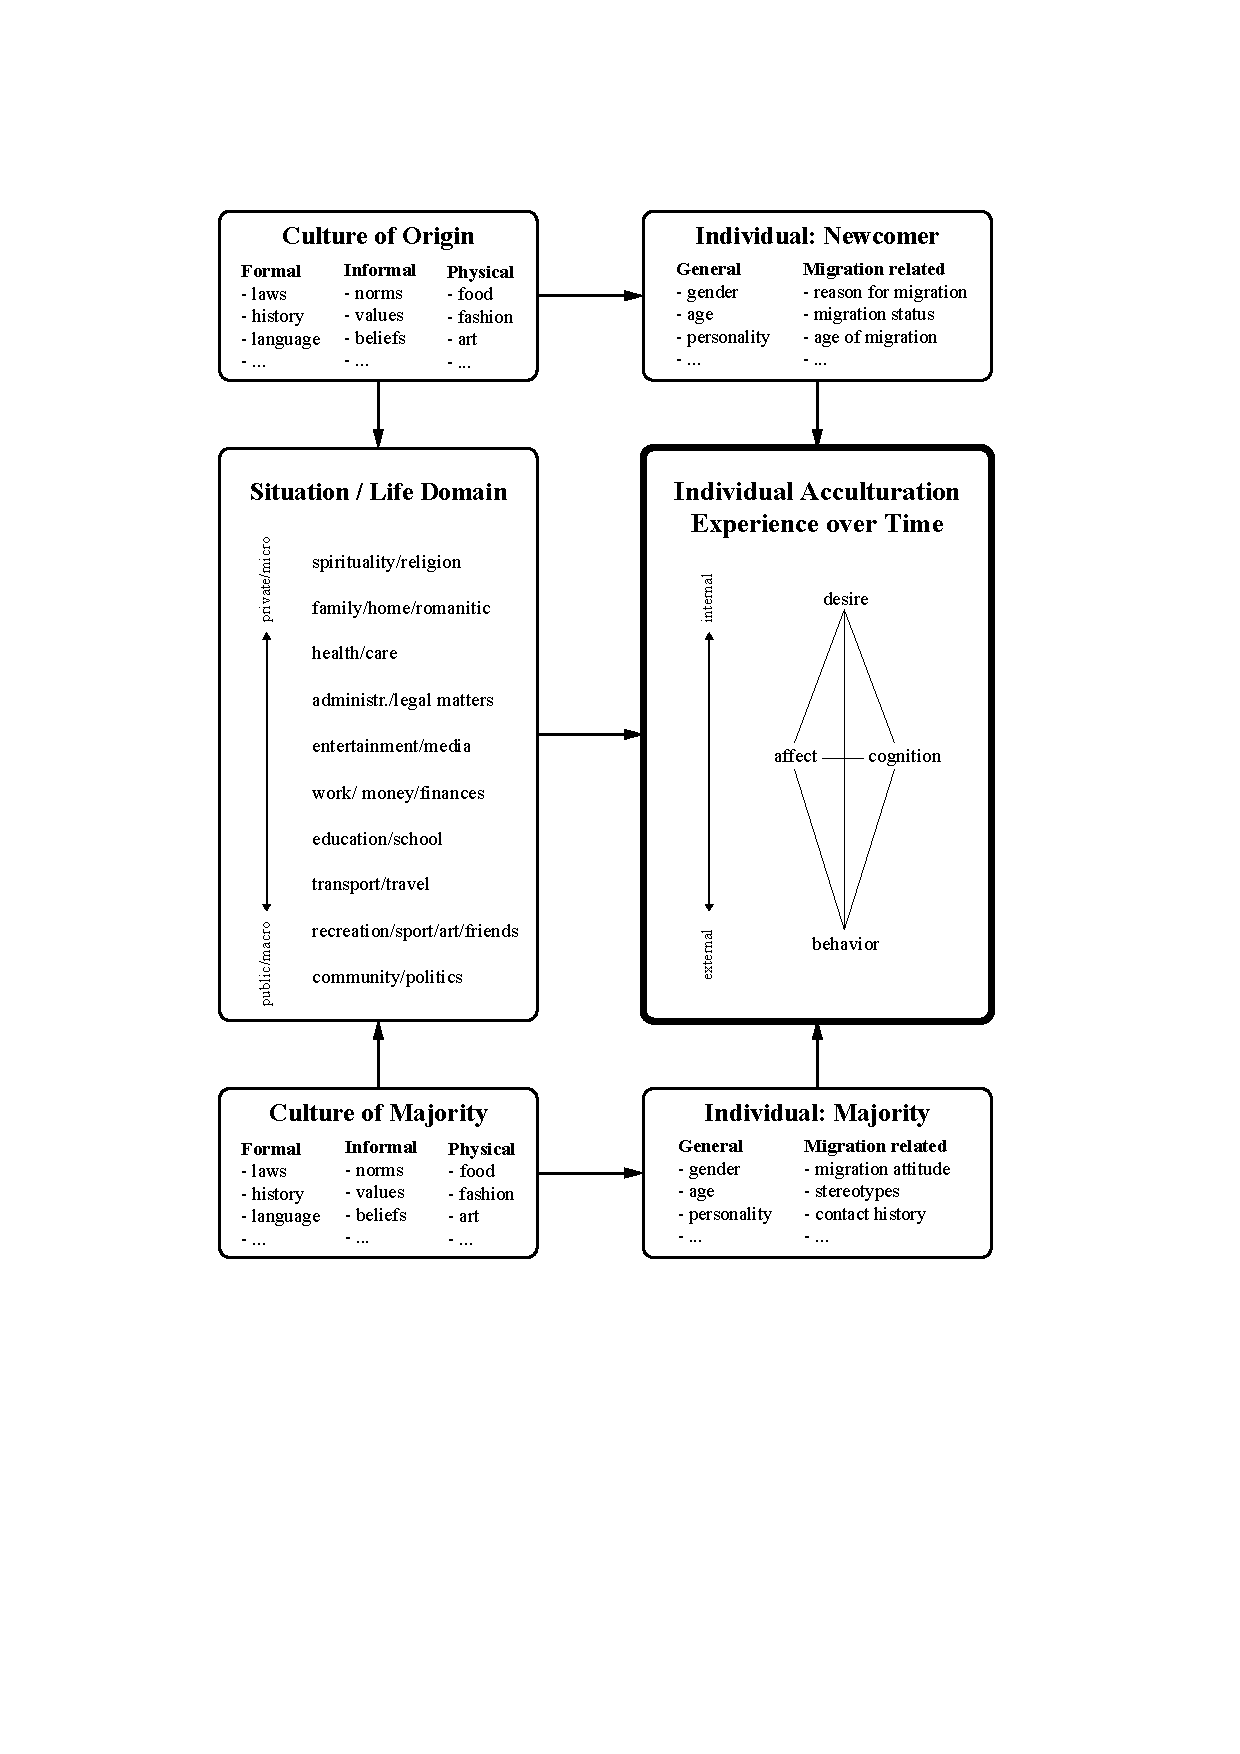
\includegraphics[width=\textwidth]{Figures/ConceptualFrameworkStatic.pdf}
\label{fig:ModelContext}
\end{figure}

\subsection{The Experience}
An experience is the process of (consciously) perceiving a life event. Although the term `experience' itself is widely discussed and contested, our psychological understanding of experiences has commonly been broken down into affects, behaviors, cognitions, and desires \citep[e.g.,][sometimes referred to as the ABCs or ABCDs of psychology]{Cottam2010, Hogg2005, Jhangiani2014}. So, from an individual psychological perspective, any experience -- including the migration experience -- can structurally be perceived as a set of motivations or goals (i.e., desire), emotions (i.e., affect), thoughts (i.e., cognition), and behaviors. At the same time, for any individual experience the content of these elements will likely differ. So while anyone will have goals, emotions, thoughts, and behaviors (i.e., experience structure), what one needs (e.g., belongingness or independence), feels (e.g., sadness or happiness), thinks (e.g., identification or disinterest), or does (e.g., studying or working) is highly ideographic (i.e., experience content). We believe that the general \textit{structure} and ideographic \textit{content}, will help organize the analysis, measurement, and understanding of individual cultural adaptation.

\subsubsection{Experience Structure}
ABC and ABCD models have been used to structure theories and models in a wide variety of fields, including research on attitudes \citep{Breckler1984} and ambivalence \citep{VanHarreveld2015}, self-regulation \citep{Ben-Eliyahu2015}, the big five personality traits \citep{Wilt2016}, suicidality \citep{Harris2015}, and even in the review of acculturation literature \citep{Ward2001, Ward2019}. The ABC(D) frameworks have also been found across cultures \citep[e.g.,][]{Bhawuk2011}, used in clinical interventions \citep{Eifert1989}, been proposed as a framework of forebrain functioning \citep{Swanson2020}, and the development of human-like machines \citep{Guo2020}.

% too much repetition (combine two sentences?) or okay?
Following the premise that any human experience will be perceived as a set of motivations or goals (i.e., desire), emotions (i.e., affect), thoughts (i.e., cognition), and behaviors, we suggest that the migration experience can also be understood within these four elements. If these four elements, indeed, capture the migration experience sufficiently, such a framework could be used to structure the assessment and understanding of conceptual definitions and measurements. Cultural adaptation might, for example, be understood or measured in terms of behavioral adaptation, such as language use, or voting; cognitive adaptation, such as identification with cultural values; affective adaptation, such as feeling at home, or loneliness; motivational adaptation, such as the satisfaction of competence or independence needs; or as a complex combination of any or all of these aspects. 

Because motivations, emotions, thoughts, and behaviors are what \citet{Berry2009a} refers to as ``basic psychological processes and capacities'' (p. 362) these elements are relevant to any human being -- across cultural, individual, situational, and temporal contexts; and these perceptions are scaleable evaluations -- of a single situation, a recent period, or a life-long journey. This is ideal for comparing and assessing different definitions and measurements in past and present literature. It allows us to ask questions such as: Which aspect of the migration experience has been considered as part of acculturation in a particular research project? Which aspect is measured most frequently in a certain field? What is the average number of aspects included in definitions or measurements? 
In the current paper, we will test some of these questions for the past empirical literature. In particular, we will assess which aspects of cultural adaptation have most frequently been included. And which aspects most frequently are included (or excluded) together. We will also assess the complexity of the measurements -- that is how many of the motivational, emotional, cognitive, and behavioral aspects have been included. To assess differences between fields, we will also group past research based on the journals' target audience. And to assess changes over time, will assess the development of the conceptual composition based on the year of publications. [\Warning\ @self: re-check after analysis write-up]
% interesting: call for unpublished data or check in theses, whether different ABCD composition.


Moreover, the structural framework also allows for novel questions and predictions. The structure, for example, allows for considerations of the relative importance, the interconnections, or the accessibility of these elements. There might, for example, be theoretical reasons why a certain aspect is more important to a specific issue (e.g., the role of emotions and cognitions to mental health; reference to theory here?). One could also offer process considerations, making theoretical arguments why a certain aspect might precede another or how one aspect might feed back into another (e.g., motivations guiding cognition and affect, which in turn drive behavior; reference to theory here? e.g., theory of reasoned goal pursuit). Another example, for a novel prediction could be a consideration of the accessibility of the individual aspects, where more public aspects, such as behaviors, might be seen as more important to the majority society, whereas more internal aspects such as motivations and goals might be more important to the newcomer (or their group; reference to theory here?). [\Warning\ maybe move to discussion?]

\subsubsection{Experience Content}
While the structure considerations so far have been content-neutral, the actual needs, feelings, thoughts, and behaviors of an experience might also be of interest. Migration is a deeply contextual and transformative experience. The influences of the host- and heritage cultures, one's personal background and psychological make up, the situational norms and environments, but also changes over time will likely influence the content of the needs, thoughts, emotions, and behaviors. 
However, there might also be structural patterns one could assess and novel questions one can ask. One might, for example, assess which emotions were most frequently included in measures and definitions of acculturation \citep[e.g., specific emotions such as anger or pride, but also types of emotions, such as positive or negative, or about yourself or others;][]{DeLeersnyder2017}. One might also be interested in co-occurences of contents (e.g., within aspect: identifications and attitudes, but also between aspects: the need for belongingness and emotion of loneliness). It would also allow for conscious considerations of relationships within or between experience aspects. And these types of questions can be asked about past definitions and measurements (i.e., are there patterns in the literature), for a specific field (e.g., which emotions are relevant in the clinical context) or a specific cultural context (e.g., are there specific needs of Syrian refugees in Europe). 

In sum, although the content and development may vary between contexts, the structuring properties (including comparability, relative importance, interconnections, and accessibility) of the fundamental aspects is unaffected by context and relevant to any experience \citep[also see][for a discussion of the distinction between \textit{universalism} and \textit{absolutism}]{Berry2000, Berry2009a}\footnote{In this paper we will at times refer to these elements of the experience as the \textit{dimensions of the migration experience}. We use the term dimensions because the importance and awareness of any of those elements likely varies between situational, cultural, individual, and temporal context. Note that these dimensions are not the same as Berry's acculturation attitude dimensions (i.e., maintenance of heritage culture, and adoption of mainstream culture; \citealp[e.g.,][]{Berry1989}).}.
More generally, such considerations of structure and content might also allow for a more nuanced understanding of what we mean to entail when we refer to acculturation, or cultural adaptation. Such considerations would also afford a more informed decision on what to include or exclude in future studies or interventions.

\subsection{The Context}
The perceptions of an experience are often fundamentally influenced by the context and environment. Which perceptions a situation permits (i.e., contextual affordances) has long been a topic of discussion in the field of ecological psychology \citep[e.g.,][]{Cantor1994}. Recent efforts to formalize the structure of contexts have, for example, highlighted the interactive process of group-environments and individuals \citep[e.g.,][]{Young2002}.
And while we have already established that the cultural adaptation process is necessarily contextual and that within this context lies a magnificent variety of lived realities, we have yet to discuss how we conceptualize this context as part of the experience framework and in our analyses presented here. 
Adjacent to the discussions in ecological psychology, we would like to address four contextual factors in particular: (1) Cultures, (2) individuals, (3) situations, and (4) the process.

\subsubsection{Culture} 
\todo[inline]{culture: patterns of social arrangements in society \\
Note to self - Émile Durkheim: \\
institutions (family, government, economy, media, education, healthcare, and religion) and social facts (formal: law, regulations, policies, history, language; informal: norms, values, beliefs, [e.g., roles, moral-, religious beliefs], rituals, customs, cultural products: fashion, architecture, arts [e.g., film, music, literature, art])
}
The most prominent contextual factor of cultural adaptation is probably the role of the interacting cultures. The role of culture seems particularly important, because it becomes salient in our social lives and influences a wide variety of attitudes and behaviors, but also in social structures and institutions. 
Most (semi-)applied research projects might not need to consider or formalize the structural role of cultures -- because they can simply embed their research in the cultural context of the two particular cultures they considered.
But theories of acculturation and broader social- and cultural theories have long considered different conceptual influences of culture and society on the individual's experience. We will rely on these theories to guide our understanding of culture here. However, because our framework fundamentally relies on the individual acculturation experience, we will merely use the structuring elements of these sociological, anthropological, and psychological theories. Moreover, because these fields often use different terms to describe the same or similar concepts, our presentation here might not always be consistent with the original terminologies. Similarly, the individual theoretical and philosophical positions and implications (and their criticisms) would be beyond the scope of our paper and will thus not be discussed here.

In our attempt to structure the influences of \textit{culture} we will mainly use extensions on Émile Durkheim's concept of \textit{social facts} \citep[e.g.,][]{Durkheim1982, Gilbert1989} and Berry's \textit{general framework of acculturation} \citep{Berry1997b, Berry2003, Berry2006a}. Interestingly, Durkheim's original definition of the concept of social facts directly referred to affect, behavior, and cognition (and potentially desires), when he wrote that social facts ``consist of manners of acting, thinking and feeling external to the individual, which are invested with a coercive power by virtue of which they exercise control over him'' (p. 52). Following this definition, we will mainly consider external (cultural or societal) influences that guide a person's motivational, cognitive, emotional, and behavioral experience. Within the sociological literature, these social influences can be divided into the formal social facts (e.g., laws, regulations, policies, history, language), informal social facts \citep[e.g., norms, values, beliefs, rituals, customs; also see][]{Herzog2018}, as well as more material cultural products or artifacts \citep[e.g., food, fashion, architecture, or arts, such as film, music, literature, and fine arts; e.g., see][]{Alexander2001}. The content of these external influences will likely be relevant in the expected patterns of behavior (e.g., dress or communication styles), cognition (e.g., sense of race-, class-, gender-, and sexual identities), emotions (e.g., expressions of emotions), and motivations (e.g., virtues and duties).

In the case cultural adaptation (at least) two sets of cultural arrangements will be influencing the experience of the individual. Quite a substantial body of literature has considered this interaction between the two cultures. For our conceptualization we will use Berry's framework for acculturation research \citep[e.g., see][p. 15, Fig. 2]{Berry1997b} and Berry's acculturation framework for stress and adaptation \citep[e.g., see][p. 45, Fig. 4.1]{Berry2006a}, because they explicitly propose to jointly consider the cultural influences on the ``acculturation experience'', which we consider here (see Figure \ref{fig:ModelContext}). Once we consider this encounter of multiple cultures within the structure of culture as social facts, it also becomes apparent that there are usually considerable power imbalances between the cultures \citep[e.g., see][]{Bhatia2001}. This imbalance is especially apparent in formal or material elements, such as laws or language, but similarly extends to more informal elements, such as default expectations in communication or behavioral norms and customs. Factors such as cultural distance \citep{Triandis2001} or majority group's attitudes \citep[e.g.,][]{Berry1997b, Berry2003} might, of course, influence such power imbalances, but the structuring of both acculturation and culture encourages and facilitates reflections and discussions of these issues. As part of the analyses presented in this paper, we will offer such a reflection by extracting the cultures for which acculturation measures were validated and investigated in empirical papers. This allows us to examine how much the external influences of culture on motives, emotions, thoughts, and behaviors are reflected within structural differences of measures and definitions (that is, if we can consolidate a meaningful number of studies per cultural context).

\subsubsection{Individual} 
Another contextual factor to consider during the cultural adaptation process are the interacting individuals themselves. There has been a rising focus on the idea that acculturation centers around the daily interpersonal interactions a person has with people of the other group \citep{Maxwell2017, Sam2010}. And although it can, at times, be difficult to disentangle cultural from individual influences, there are a range of personal features that likely influence the cultural adaptation process. These personal differences might relate to relatively stable individual differences, such as gender or personality, but also migration related differences, such as the reason for migration (e.g., voluntary vs. forced migration), cultural distance, or migration status. Within the migration related factor we would also include aspects that might change over the course of the adaptation process but give migrants different starting positions, such as language skills and education level.
Similar to the influences of cultures, the individual differences of the interaction partners (if there are multiple people) will likely impact the cultural adaptation. And similar to culture, individual differences likely play a role for multiple aspects of the cultural adaptation process (also see Figure \ref{fig:ModelContext}). As part of this study, we will mainly analyze the migration relevant differences. Considering individual differences on a larger, cross-study, level we will mainly extract data on the type of samples collected within the validation and the empirical papers (e.g., forced vs. voluntary, youth, or clinical samples). If we find reasonable numbers of studies with specific types of samples, we will assess whether these individual differences are related to structural differences in measures or definitions used by the authors.

\subsubsection{Situation} 
\todo[inline]{The Situation (domains of psycho-social functioning)}
Beyond the cultural group and the individuals, the interactions of cultural adaptation are further dependent on the situational context. One way of structuring this situational context is what we will here refer to as the \textit{domains of psycho-social functioning} -- the idea that the social experience will take place within different domains in life. There are many social-scientific theories that have discussed these spheres of life. One famous example is Bronfenbrenner's Ecological systems theory \citep{Bronfenbrenner1992}, according to which humans get into contact with other, and society at large, through a number of environmental systems that range from the closest relations (e.g., family or colleagues) to the more remote relationships (e.g., mass media or societal services). A similar framework was suggested by prominent theorists of the (structural) functionalist traditions with the concept of social institutions \citep[e.g.,][]{Turner1997}. According to these sociological theorists, it is through societal institutions (commonly: family, government, economy, media, education, healthcare, and religion) that culture is transmitted and maintained \citep[e.g.,][]{Durkheim1982}. Similar ideas for domains of interaction with society and culture have also been proposed within the acculturation literature. \citet{Arends-Toth2006, Arends-Toth2007} have, for example, suggested 15 public and private life domains (e.g., education [public], child-rearing [private]) in which acculturation takes place. Empirical research in the individual acculturation field, have also provided evidence that acculturation processes can develop separately and differently within these domains \citep[e.g.,][]{Arends-Toth2003a}. 
%point of convergence
What structurally unites the conceptualizations of life domains is the dimension of closeness to the individual. That is, most areas of life found in the literature can be arranged from the most immediate (i.e., micro or private, such as family) to the broadest levels (i.e., macro or public, including government or media). So, based on sociological theories of social institutions \citep{Durkheim1982}, literature on life domains in acculturation \citep{Arends-Toth2006, Arends-Toth2007, Zane2004}, a categorization of psychological influences by the British Psychological Society \citep{Michie2005a}, and Bronfenbrenner's Ecological systems theory \citep{Bronfenbrenner1992}, we conceptualized a range of life domains relevant to the migration process (see Figure \ref{fig:ModelContext}). Interestingly, most methodological and empirical authors mention explicitly which domains of acculturation they measure or very clearly focus on a limited number of domains in their measurement or definition of acculturation. As part of this study we will, therefore, extract information on the domains mentioned and measured in the literature. We will then assess whether different foci on life domains also show differences in their understanding and measurement of the motivational, emotional, cognitive, and behavioral cultural adaptation.

\subsubsection{Process} 
A final, fundamental factor we would like to address in the cultural adaptation framework the understanding of cultural adaptation as a dynamic process rather than a static end-product. That cultural adaptation is a developmental process, and that ``acculturation occurs when two independent cultural groups come into \textit{continuous first-hand contact over an extended period of time}'' \citep[][186]{Berry1989} seem to be a generally accepted assumption within the field. Yet, within the empirical literature, few studies have actually considered the theoretical implications of migration as a process and even fewer have methodologically followed the trajectories of migrants over time. Recent years have seen a growing awareness of this discrepancy \citep[e.g.,][]{Brown2011, Ward2019}. We believe that the experience framework of cultural adaptation, as it is presented here, is ideally suited to deal with this conceptualization as a developmental process. Philosophers of the phenomenological tradition have long highlighted that subjective experience can only be understood within the history of past experiences \citep[e.g.,][; also see Figure \ref{fig:ModelContext}]{Heidegger1867}. In this study we apply our interest in the role of time by extracting the types of analyses (static vs. dynamic) done by the authors, and assessing whether data was collected prior to migration, after migration, or both. We will then also assess whether different traditions of data collection show differences in their understanding and measurement of the motivations, emotions, thoughts, and behaviors aspects of cultural adaptation (if the systematic review includes a reasonable number of longitudinal studies).

\subsubsection{Bottom-up Approach} 
One further strength of the experience concept is that it highlights the considerations for the lived realities of the researched individuals and communities. Scholars in the traditions of critical research methods have long highlighted the importance of including the participants in the research conceptualization process \citep[e.g.,][]{Kovach2009}. If one uses the perspectives of the researched individuals to guide the study questions and design, one inevitably emphasizes the agency and needs of the community -- lending relevance and ownership of knowledge to the community \citep[e.g., ][]{Schmidt2021}.

Before we move on to the systematic review and our test of the conceptual framework, we would like to remark on our focus on the migrant's rather than the majority group member's experiences. 
While this framework explicitly focuses on the migrant's experience as the structuring experience, this is not meant to put the sole responsibility of ``migration success'' on the newcomer or ignore the interconnectedness of intercultural exchange. We focus on the migrant experience as the structuring element because migrants usually find themselves in disadvantaged positions. 
We would also like to address the issue of interactive acculturation. \citet{Bourhis1997a} and others, have often highlighted that cultural adaptation is essentially interactive and one should not consider the acculturation process of one individual or group without the consideration of the other group and the interaction partners. We agree, and while we address some of these issues explicitly in the framework, we would also like to highlight that within the experience framework aspects of cultural adaptation that are interconnected, co-dependent, or depend on the host majority members likely influence the individual's migration experience. As an example, if a migrant is frequently confronted with exclusion and hostility, this will likely affect their motivations, emotions, thoughts, and behaviors. 
We would also like to highlight that the framework is equally applicable to the cultural adaptation experience of host majority members in their interactions with or perceptions of migrants. Although not the focus of this paper, the same assessments of measures, definitions, and understandings should be able to be conducted with the experience of the majority group.
Additionally, this framework is not meant as an exhaustive or exclusive list of all adaptation aspects but rather offers a structural framework to analyze and understand the broad experience of cultural adaptation.
%Migration is a complex trans-formative experience within different areas of personal- and social life. 

\subsection{The present study}

\Warning Should we move all the ``In this study ...'' parts into this section? \\
\noindent I like both. In the current version, there is always immediately a bridge back to our research, but if we bundle them here and have the upper section on the model only it might be easier to know what to expect. We could also do both? Have them in short up in the model part and then reiterate the \textit{aims} here, similar to a hypotheses section.

One paragraph on the aims of our analyses.

One paragraph on the structure of the paper.

\begin{enumerate}
  \item \sout{More on past Literature on conceptualization and measurement (?)}
  %\item Focus group discussion
  \item Systematic review
   \begin{enumerate}
     \item methodological literature
     \item empirical literature
   \end{enumerate}
   \item Potentially Paragraph on: Why not meta analysis (too diverse and scattered; main problem comparability across studies).
 \end{enumerate}


\section{Systematic Review}
We conducted a systematic review of the past literature. By analysing the domains and dimensions represented and measured in the academic literature we (1) test the utility of the framework, (2) gain an overview of the field (incl. open potential), (3) build a database of measurements and results structured by human experience and motivation.

For the coding, we individually consider methodological and empirical work. In a first step, we analyse validated scales reported in reviews as well as the empirical papers. In a second step, we consider the full body of empirical work.

\subsection{Coding}
\subsubsection{Dimensions}
One major focus of our coding efforts was identifying the phenomenological dimensions that were assessed by each individual scale. Examples of how we distinguished between emotional (affect), behavioural, cognitive, and need-based measurements of acculturation are in Table \ref{tab:DimensionExamples}.
\begin{table}[hbt]
\caption{Examples for Dimensions of Acculturation Coding}
\label{tab:DimensionExamples} 
\begin{tabular}{lll}
\hline
Dimension & Concept & Wording \\ 
\hline
Affect & belonging, loneliness, satisfaction  & "I feel ...", \\
Behavior  & \begin{tabular}[c]{@{}l@{}}language learning, media consumption,\\ 
voting\end{tabular} & "I do ...", "I speak ...", "I meet ..." \\ 
Cognition & \begin{tabular}[c]{@{}l@{}}cultural identification, cultural values,\\ 
attitude towards majority\end{tabular} & \begin{tabular}[c]{@{}l@{}}"I prefer ...", "I think ...", \\
"I identify as ..."\end{tabular} \\ 
Desire    & needs, goals, wants & \begin{tabular}[c]{@{}l@{}}"I want ...", "I would like to ...", \\
"I need ..."\end{tabular} \\ 
\hline
\end{tabular}
\end{table}


Table \ref{tab:ScaleTbl}.

\begin{longtable}[l]{lclclclclclc}
\caption{(\#tab:ScaleTbl)Cultural Adaptation Scales}\\
\toprule
Scale & Reference & Source \footnote[1]{CEL = @Celenk2011, MAE = @Maestas2000, MAT = @Matsudaira2006, WAL = @Wallace2010, ZAN = @Zane2004, OWN = own review (only additional)}" & Affect & Behavior & Cognition & Desire & domainScale & Sample & IncludesMajority & HostCountry & OriginCountry\\
\midrule
\endfirsthead
\caption[]{(\#tab:ScaleTbl)Cultural Adaptation Scales \textit{(continued)}}\\
\toprule
Scale & Reference & Source \footnote[1]{CEL = @Celenk2011, MAE = @Maestas2000, MAT = @Matsudaira2006, WAL = @Wallace2010, ZAN = @Zane2004, OWN = own review (only additional)}" & Affect & Behavior & Cognition & Desire & domainScale & Sample & IncludesMajority & HostCountry & OriginCountry\\
\midrule
\endhead

\endfoot
\bottomrule
\endlastfoot
Abbreviated Multidimensional Acculturation Scale & @Zea2003 & CEL; MAT; WAL & 1 & 1 & 1 & 0 & cultural identiy, language, cultural knowledge, food consumption & general & 0 & United States of America & Latinx\\
Acculturation Attitude Scale (Safdar, Struthers, \& van Oudenhoven, 2009) & @Safdar2009 & OWN & 0 & 1 & 1 & 0 & general & general & 0 & United States of America, Netherlands, United Kingdom & Iran\\
acculturation attitudes (Arends-Tóth \& van de Vijver, 2007) & @Arends-Toth2007 & OWN & 0 & 1 & 1 & 0 & Private domain (celebrations, eating food, child-rearing practices, cultural habits, cultural way oflife, self-reported cultural identity, and attributed cultural identity as seen by the respondent). Public domain (social contacts, friends at school, speaking the language, reading the language, education and courses, teachers, news and information, and reading newspapers). & general & 0 & Netherlands & Turkey\\
Acculturation Attitudes Scale (Sam \& Berry, 1995) & @Sam1995 & CEL; MAT & 1 & 1 & 1 & 1 & general & youth & 0 & Norway & Third World\\
Acculturation Attitudes Scale-Revised & @Berry2010 & CEL & 1 & 1 & 1 & 1 & identity & general & 1 & multiple & multiple\\
Acculturation Index (Ward \& Kennedy, 1994) & @Ward1994 & MAT & 0 & 1 & 1 & 0 & general & general & 0 & any & New Zealand\\
Acculturation Index (Ward \& Rana-Deuba, 1999) & @Ward1999 & CEL & 0 & 1 & 1 & 0 & clothing, pace of life, general knowledge, food, religious beliefs, material comfort, recreational activities, self-identity, family life, accommodation/residence, values, friendships, communication styles, cultural activities, language, employment activities, perceptions of co-nationals, perceptions of hertiage/host nationals, political ideology, worldview, social customs & general & 0 & Nepal & any\\
Acculturation Orientation (based on Horenczyk, 1996, 2000) & @Ben-Shalom2003 & OWN & 1 & 0 & 1 & 1 & language, friendship, culture & soldiers & 0 & Israel & former Soviet Union\\
Acculturation Questionnaire for Children & @VanDeVijver1999 & MAT & 0 & 1 & 1 & 0 & books, learning more about a country, ethnicity of friends, importance of speaking a language, affinity to a language, place to live, ethnicity of teacher, place to work later in life, food, and games & youth & 0 & Netherlands & any\\
Acculturation Rating Scale for Arab-American-II & @Jadalla2013 & OWN & 1 & 1 & 1 & 0 & general & general & 0 & United States of America & Arabic Countries\\
Acculturation Rating Scale for Mexican Americans & @Cuellar1980 & CEL; MAE; MAT; WAL; ZAN & 0 & 1 & 1 & 0 & general & clinical & 0 & United States of America & Mexico\\
Acculturation Rating Scale for Mexican Americans–II & @Cuellar1995a & CEL; MAE; MAT; WAL; ZAN & 1 & 1 & 1 & 0 & general & students & 1 & United States of America & Mexico\\
Acculturation Rating Scale for Mexican Americans–Short Form & @Dawson1996 & CEL; MAE; WAL & 0 & 1 & 1 & 0 & general & general & 0 & United States of America & Hispanic\\
Acculturation Scale (Arends-Tóth \& van de Vijver, 2000) & @Arends-Toth2000 & OWN & 0 & 1 & 1 & 0 & contact, upbringing, language, culture, education & general & 1 & Netherlands & any\\
Acculturation Scale (Cheung, 1995) & @Cheung1995 & OWN & 1 & 1 & 1 & 1 & language use, customs, cultural value, perceived discrimination, sociability & general & 0 & New Zealand & Cambodia\\
Acculturation Scale (Ghuman, 1991) & @Ghuman1991 & MAT & 1 & 0 & 1 & 1 & food, clothing, the role of women, religion, entertainment, community life & youth & 0 & United Kingdom & any\\
Acculturation Scale (Ghuman, 1997) & @Ghuman1997 & CEL & 0 & 0 & 1 & 1 & equality of sexes, dating and marriage, living within ethnic enclaves, learning of a community language, attending mosques and watching Asian films. & youth & 0 & United Kingdom & India\\
Acculturation Scale (Ghuman, 2000) & @Ghuman2000 & MAT & 0 & 0 & 1 & 1 & equality of sexes, dating and marriage, living within ethnic enclaves, learning of a community language, attending mosques and watching Asian films. & youth & 0 & Australia & South Asia\\
Acculturation Scale for Southeast Asians & @Anderson1993 & MAE; MAT; ZAN & 0 & 1 & 1 & 0 & language, food preference & general & 0 & United States of America & Southeast Asia\\
Acculturation Scale for Vietnamese Adolescents & @Nguyen2002 & CEL; MAE; MAT & 1 & 1 & 1 & 1 & group interactions, everyday lifestyle, family orientation, global involvement & youth & 0 & United States of America & Vietnam\\
Acculturation, Habits, and Interests Multicultural Scale for Adolescents & @Unger2002 & CEL; WAL & 1 & 1 & 1 & 0 & friends, family activities, entertainment media & youth & 1 & United States of America & any\\
Acculturative Hassles & @Vinokurov2002 & CEL & 0 & 1 & 0 & 0 & discrimination, peer, language, family & refugee & 0 & Russia, United States of America & former Soviet Union\\
Acculturative Stress Inventory for Children & @Suarez-Morales2007 & CEL & 1 & 1 & 1 & 0 & stress (neg.) & youth & 0 & United States of America & Hispanic\\
Acculturative Stress Scale & @DeSnyder1987a & CEL & 1 & 1 & 1 & 0 & familial, marital, social, financial, and environmental & general & 0 & United States of America & Mexico\\
Adopt and Keep Scale & @Swaidan2006 & CEL & 0 & 1 & 1 & 0 & general & general & 0 & United States of America & Middle East, Asia\\
American and Puerto Rican Cultural Involvement Scales & @Cortes1994 & MAT; WAL & 1 & 0 & 1 & 0 & general & general & 0 & United States of America & Puerto Rico\\
Asian American Multidimensional Acculturation Scale & @GimChung2004 & CEL; MAT & 1 & 1 & 1 & 1 & cultural identiy, language, cultural knowledge, food consumption & students & 0 & United States of America & Asia, South Korea\\
Asian Values Scale & @Kim1999 & MAT; ZAN & 0 & 0 & 1 & 0 & values & students & 1 & United States of America & Asia\\
Behavioral Acculturation Scale & @Szapocznik1978 & MAE; MAT; ZAN & 0 & 1 & 1 & 1 & language, daily customs and habits, idealized lifestyle & general & 1 & United States of America & Cuba\\
Bicultural Identity Integration Scale (BIIS-1) & @Benet-Martinez2005 & CEL & 1 & 0 & 1 & 0 & cultural identity & general & 0 & United States of America & China\\
Bicultural Identity Integration Scale (BIIS-2) & @Huynh2018 & CEL & 1 & 0 & 1 & 0 & cultural identity & students & 0 & United States of America & any\\
Bicultural Involvement Questionnaire & @Szapocznik1980 & CEL; MAT; ZAN & 1 & 0 & 0 & 1 & language, daily customs and habits, idealized lifestyle & youth & 0 & United States of America & Cuba, Hispanic\\
Biculturalism/Multiculturalism Experience Inventory & @Ramirez1983 & MAT; ZAN & 1 & 1 & 0 & 0 & socialization and educational experiences, interpersonal interactions, and experiences in situations related to school, political, athletic, religious, family, and recreational spheres & general & 0 & United States of America & Hispanic\\
Bidimensional Acculturation Scale & @Jang2007 & OWN & 1 & 1 & 1 & 0 & language, media consumption, food consumption, social relations, sense of belonging, and familiarity with culture & general & 0 & United States of America & South Korea\\
Bidimensional Acculturation Scale for Hispanics & @Marin1996 & CEL; MAE; MAT; WAL; ZAN & 1 & 1 & 0 & 0 & language use, language proficiency, media & general & 0 & United States of America & Hispanic\\
Brief Acculturation Scale & @Meredith2000 & CEL; MAE; MAT & 0 & 1 & 1 & 0 & language, identity & general & 0 & United States of America & Japan\\
Brief Acculturation Scale for Hispanics & @Norris1996 & CEL; MAT; WAL; ZAN & 1 & 1 & 0 & 0 & language, closeness & youth & 0 & United States of America & Hispanic\\
Chicano Adolescent Acculturation Scale & @Olmedo1978a & MAE; WAL & 0 & 0 & 1 & 0 & general & youth & 1 & United States of America & Mexico\\
Children’s Acculturation Scale & @Franco1983 & CEL; MAE; MAT; ZAN & 0 & 1 & 1 & 0 & general & youth & 0 & United States of America & Mexico\\
Children’s Hispanic Background Scale & @Martinez1984 & CEL; WAL; ZAN & 0 & 1 & 1 & 0 & language use, food preference, cultural exposure & youth & 0 & United States of America & Mexico\\
Cultural Health Attributions Questionnaire & @Murguia2000 & WAL & 0 & 0 & 1 & 0 & cultural health beliefs & general & 0 & United States of America & Hispanic\\
Cultural Life Styles Inventory & @Mendoza1989 & CEL; MAE; MAT; ZAN & 1 & 1 & 1 & 0 & language use, extrafamilial language use, so-cial affiliation, cultural familiarity, and cultural identification and pride & general & 1 & United States of America & Mexico\\
Cultural Readjustment Rating Questionnaire & @Spradley1972 & CEL & 1 & 1 & 1 & 0 & general & students & 1 & United States of America & China\\
Cultural Values Conflict Scale & @Inman2001 & MAT & 1 & 1 & 1 & 1 & dating/premarital sexual relations;, marriage, family relations, sex role expectations, communality estimates & women & 0 & United States of America & South Asia\\
Culture Shock Questionnaire & @Mumford1998 & CEL & 1 & 1 & 1 & 1 & stress & general & 0 & any & United Kingdom\\
East Asian Acculturation Measure & @Barry2001a & OWN & 1 & 1 & 1 & 0 & general & general & 0 & United States of America & China, Japan, South Korea\\
European American Value Scale for Asian Americans & @Wolfe2001 & MAT & 0 & 0 & 1 & 0 & values & students & 1 & United States of America & Asia\\
General Ethnicity Questionnaire (Tsai, Ying, \& Lee 2000) & @Tsai2000 & CEL & 1 & 1 & 1 & 1 & language use and proficiency, affiliation with people, participation in activities, pride in culture, exposure to culture, and preference for food & students & 0 & United States of America & China\\
Greek-American Acculturation Scale & @Harris1996 & MAT & 1 & 1 & 1 & 1 & language, values, identification, comfort, pride & general & 1 & United States of America & Greece\\
Hazuda Scale & @Hazuda1988 & MAT & 0 & 1 & 1 & 0 & language, cultural practices, family structure & general & 1 & United States of America & Mexico\\
Homesickness and Contentment Scale & @Shin1999 & CEL & 1 & 1 & 1 & 1 & general & students & 0 & United States of America & China, South Korea\\
Immigrant Acculturation Scale & @Madianos2008 & OWN & 0 & 1 & 1 & 0 & general & general & 0 & Greece & any\\
Integration Efforts & @Guest1993 & OWN & 0 & 1 & 0 & 0 & Social, residential, personal & general & 0 & United States of America & any\\
Intercultural Adjustment Potential Scale (ICAPS) & @Matsumoto2001 & OWN & 1 & 1 & 1 & 0 & Emotional regulation, Openness, Flexibility, Creativity & general & 0 & United States of America & Japan\\
Internal-External Ethnic Identity Measure & @Kwan1997 & CEL & 0 & 1 & 1 & 1 & food, damily, social contacts, community, values & general & 0 & United States of America & China\\
Italian Ethnic Identity Measure & @Laroche2005 & CEL & 0 & 1 & 1 & 0 & language, media, family, attachment & general & 0 & Canada & Italy\\
Italian-Canadian Acculturation Scale (Kim, Laroche, \& Tomiuk, 2001) & @Kim2001 & OWN & 1 & 1 & 1 & 0 & language use, mass media exposure, social interactions, identification, attachment & general & 0 & Canada & Italy\\
Language-based Acculturation Scale & @Deyo1985 & CEL; MAT & 0 & 1 & 1 & 0 & language & clinical & 0 & United States of America & Mexico\\
Language, Identity, and Behavioral Acculturation Scale & @Birman2002 & OWN & 0 & 1 & 1 & 0 & general & refugee students & 0 & United States of America & former Soviet Union\\
Latino/Latina Acculturation Scale & @Felix-Ortiz1994 & WAL & 0 & 1 & 1 & 0 & value/attitude, Perceived Discrimination, Feminism, Respeto, Activism, Affiliation; Familiarity with Culture, Language Preference, Language Proficiency & students & 0 & United States of America & Latinx\\
Los Angeles Epidemiologic Catchment Area-Acculturation Scale & @Burnam1987 & MAE; WAL & 0 & 1 & 0 & 0 & language familiarity and usage, ethnic interaction, activities reflecting cultural traditions and lifestyle, ethnic identification, ethnic background & general & 0 & United States of America & Mexico\\
Media Acculturation Scale & @Ramirez1986 & CEL; WAL; ZAN & 0 & 1 & 0 & 0 & language & general & 0 & United States of America & Mexico\\
Mexican American Acculturation Scale & @Montgomery1992 & MAE; WAL & 1 & 1 & 1 & 0 & general & students & 1 & United States of America & Mexico\\
Multicultural Acculturation Scale & @Wong-Rieger1987 & MAT & 1 & 1 & 1 & 0 & general & general & 1 & United States of America & Southeast Asia, Latinx\\
Multidimensional Acculturative Stress Inventory & @Rodriguez2002 & CEL & 1 & 1 & 1 & 0 & general & general & 0 & United States of America & Mexico\\
Multidimensional Acculturative Stress Scale & @Jibeen2010 & CEL & 1 & 1 & 1 & 0 & Discrimination, Ethnic Identity, work,  Homesickness, Language & general & 0 & Canada & Pakistan\\
Multigroup Ethnic Identity Measure & @Phinney1992 & OWN & 1 & 1 & 1 & 0 & identity & students & 0 & United States of America & any\\
Multiphasic Assessment of Cultural Constructs & @Cuellar1995 & MAT; WAL & 1 & 1 & 1 & 0 & values, beliefs & students & 0 & United States of America & Mexico\\
Pan-Acculturation Scale (Soriano, 1999) & @Soriano1999 & OWN & 1 & 1 & 1 & 0 & Language use, values and beliefs, social environment, ethnic identity, cultural traditions and practices & youth & 0 & United States of America & Latinx\\
Psychological Acculturation Scale & @Tropp1999 & CEL; MAE; MAT & 1 & 0 & 1 & 0 & general & general & 0 & United States of America & Latinx\\
Relative Acculturation Extended Model Scale (real and ideal acculturation strategies and attitudes) & @Navas2007 & OWN & 0 & 1 & 1 & 1 & work, economic, social relations, family relations, religion, and ways of thinking & general & 1 & Spain & Morocco, Sub-Saharan Africa\\
Satisfaction With Migration Life Scale & @Neto2016 & OWN & 1 & 0 & 1 & 1 & life satisfaction & general & 0 & United States of America & any\\
Scale of Acculturation & @Rissel1997 & CEL; MAT & 0 & 1 & 1 & 0 & language, identity & general & 0 & Australia & Arabic Speaking\\
Short Acculturation Scale & @Wallen2002 & CEL; WAL & 1 & 1 & 1 & 0 & language & women & 0 & United States of America & Central America\\
Short Acculturation Scale for Filipino Americans & @Cruz2000 & MAT & 0 & 1 & 1 & 1 & language, social interaction, children & experts & 0 & United States of America & Philippines\\
Short Acculturation Scale for Hispanic Youth & @Barona1994 & CEL; MAE; WAL & 0 & 1 & 1 & 0 & language, social interaction & youth & 1 & United States of America & Hispanic\\
Short Acculturation Scale for Hispanics & @Marin1987 & CEL; MAE; MAT; WAL; ZAN & 0 & 1 & 1 & 1 & Language Use, Media, Ethnic Social Relations & general & 1 & United States of America & Hispanic\\
Sociocultural Adaptation Scale & @Ward1994 & CEL & 0 & 1 & 1 & 0 & general & general & 0 & any & New Zealand\\
Spheres of sociocultural adjustment & @Lissitsa2011 & OWN & 1 & 1 & 1 & 1 & Current socio-economic status, host culture, host identification, Affinity to hertitage culture, Housing, Social relations, Children’s schooling, Psychological integration, Basic language proficiency, Political integration, Preservation of socio-economic status, Adopting host life style & general & 1 & Israel & Russia\\
Stephenson Multigroup Acculturation Scale & @Stephenson2000 & CEL; MAT; ZAN & 1 & 1 & 1 & 0 & language, interaction, media, food & general & 0 & United States of America & any\\
Strategies of Acculturation Scale & @Eshel2000 & OWN & 1 & 1 & 0 & 1 & general & youth & 0 & Israel & Russia\\
Suinn-Lew Asian Self-Identity Acculturation Scale & @Suinn1992 & CEL; MAE; MAT; ZAN & 1 & 1 & 1 & 0 & language choice, identity, friendship choice, acculturative behaviours, generation/geographic background, and attitudes & students & 0 & United States of America & Asia\\
Taiwan Aboriginal Acculturation Scale & @Cheng1995 & MAT & 1 & 1 & 1 & 1 & general & general & 0 & Taiwan & East Asia \& Pacific\\
Trinity Acculturation Scale & @Curran2003 & OWN & 1 & 1 & 1 & 1 & general & general & 0 & United Kingdom & Ireland\\
Value Acculturation Scale & @Szapocznik1978 & MAE; MAT; ZAN & 0 & 0 & 1 & 0 & values & general & 1 & United States of America & Cuba\\
Vancouver Index of Acculturation & @Ryder2000 & CEL; MAT & 1 & 1 & 1 & 0 & values, social relationships, traditions, entertainment & general & 1 & Canada & China\\
Virgin Island Acculturation Scale (Tull, Ambrose, \& Chambers, 2003) & @Tull2003 & OWN & 0 & 1 & 1 & 0 & government responsibility, holiday celebrations, economic principles, child rearing practices, social customs, sporting & general & 0 & United States Virgin Islands & African Cribbean\\*
\end{longtable}


Note that this also means that we do not include scales that measure aspects of acculturation that do can be measured without consideration of the individual’s experiences, such as physical changes, cultural changes, or societal changes.
\subsubsection{Domains/Context}
We coded which life domains the scales referred to, either as part of sub-scale labels, factor labels, explicit commentary of the authors, or clear question wordings.

We process the domains as a list of domains for each validation. We later assess the lists as a whole (e.g., number, diversity of domains) but also the domains individually (e.g., frequency of domain across all articles).

\subsection{Methodological Literature}
\todo[inline]{*Database Description*} 
The first data set we assess is a database of scale validations. We bring together the scales suggested in previous reviews as well as validation studies we identified in our own review. Throughout our literature review we found five major works that reviewed the measurement of acculturation \citep{Celenk2011, Maestas2000, Matsudaira2006, Wallace2010, Zane2004}.

\subsubsection{Methods}
We collected XXX scales of which XX were excluded due to main reasons. We coded dimensions and domains, but also information on the sample targeted for validation, the type of measurement, as well as the year of publication.

type of measurement (e.g., continuous, categorical)
\subsubsection{Sample}
types of sample targeted (e.g., clinical, refugees, …), and whether majority sample was included

country targets of migrants and host societies

interest over time (when were the validations published)
\subsubsection{Domains/Context}
A relatively large number of scales ask about the current state of the migrant in general manner without mentioning any context or life domain (example item here; XX\% [currently coded as 'general‘]).

The remaining scales referred to an average of X.XX dimensions (SD = X.XX). A total of XXX unique domains was measured across the XXX scales. The dimensions of ‘language‘, ‘food’, ‘interactions’, ‘family’ and ‘values’ are focussed on most often (see Online Supplementary Materials X, Figure X).

Conclusion: Large variation between the scales in the number, diversity, and consideration of domains. Most of the mentioned domains are in line with the topics proposed in the literature.
\subsubsection{Dimensions}
Most studies included a measure of cognition (XX\%) and behavior (XX\%), whereas only roughly half the studies included a measure of affect (XX\%) and only a fourth of the scales included a measure of motives (XX\%).

A minority of scales included only a single dimension (XX\% cognition only, XX\% behavior only) or all four dimensions (XX\%). Most studies measured two (XX\%) or three (XX\%) dimensions.

Co-occurrence numbers: percentage of concept in unique combinations. Which dimension is represented how much in each of the levels of complexity (k-way co-occurrences).

Conclusion: (1) most scales measure multiple dimensions and (2) focus on easily accessible dimensions (behavior and cognition), less of what is considered ``less accessible'' or ``subjective''.

\subsection{Empirical Literature}
After analysis of the scales validations, we assessed the empirical papers we collected within the systematic review. We first look at all available empirical publications (incl. books, chapters, and dissertations). We later also assessed differences between fields the work was published in. However, because we considered the fields on an audience level, we used only empirical journal articles - for which journal-level audience data is available.
\subsubsection{Methods}
Search terms (incl. inclusion and exclusion),

screening (title screening, abstract screening, full text analysis) [use \href{http://prisma-statement.org/PRISMAStatement/FlowDiagram}{PRISMA}]

We again coded domains, dimensions, sample information (sample target, country targets), publication type, and year of publication.

We additionally capture (1) which term the authors use to refer to cultural adaptation (e.g., acculturation, integration, cultural adjustment), (2) what the thematic focus of the paper is (e.g., focus on adaptation itself or other focus such as health, intergroup relations), (3) the empirical method used (e.g., quantitative, qualitative), (4) information on the analyses used (incl. where in the model the concept of placed in the main analysis).
\subsubsection{Sample Descriptives}
sample type (incl. majority inclusion, and migration time)

countries
\subsubsection{Study Descriptives}
publication types (frequencies of articles, chapters, dissertations)

term used (most common terms)

focus of the paper (most common foci)

method (frequencies of quantitative, qualitative, mixed methods)

interest over time (based on year of publication, incl. impact metrics of journal articles)

analysis and place in the model (e.g., IV, DV)

journal keywords of journal articles
\subsubsection{Domains/Context}
A relatively large number of studies assess cultural adaption in general manner without mentioning any context or life domain (XX\% [currently coded as 'general‘]).

The remaining studies referred to an average of X.XX dimensions (SD = X.XX). A total of XXX unique domains was measured across the XXX studies. The dimensions of ‘language‘, ‘food’, ‘social interactions’, and ‘friends’ are focused on most often (see Online Supplementary Materials X, Figure X).

\textbf{Conclusion}: An even larger proportion of studies remove context and ask about general levels (compared to the validation). When domains are specified the there is large variation between in the number, diversity, and discussion of the domains.

\subsubsection{Dimensions}
Most studies included a measure of cognition (XX\%) and behavior (XX\%), whereas only roughly half the studies included a measure of affect (XX\%) and only a quarter of the scales included a measure of motives (XX\%).

A minority of scales included only a single dimension (XX\% cognition only, XX\% behavior only, XX\% affect only) or all four dimensions (XX\%). Most studies measured two (XX\%) or three (XX\%) dimensions.

Co-occurrence numbers: percentage of concept in unique combinations. Which dimension is represented how much in each of the levels of complexity (k-way co-occurrences).

\textbf{Conclusion}: Interestingly, not a single study measured only motivation, and measures of desires remained mostly limited to scales that were already multidimensional (i.e., complex scales only). The results exacerbate the pattern found in the scale validations, complex measures and conceptions of acculturation are seen infrequently and readily accessible (i.e., less subjective) dimensions of cognition and behavior remain the focus of most studies.

\subsubsection{Fields}
merging and exclusions: information on the Scimago database (only data available for journals).

condensed to four mutually exclusive field codes: ‘Psychology’, ‘Medicine, Nursing, \& Health’, ‘Social Sciences (miscellaneous)‘, ‘Multidisciplinary / Cross-disciplinary‘.

short: sample descriptives by fields

short: study descriptives by field

domains (mean, sd, diversity)

dimensions (mean, sd, overall percentages, complexity, field foci)

\textbf{Conclusion}: More domain diversity for psychology and multidisciplinary (less for medical and social sciences). Cultural adaptation more often predictor (rather than outcome) for medical and psychological journals. Interestingly in psychological journals adaptation more often predictor than outcome even though focus of the paper still predominantly adaptation. Less dimension complexity and variation for medical and social science fields. Psychological highest average complexity and only XX% single dimensional measurements.

\section{Discussion}
\todo[inline]{*Summary*}
%Focus group discussion: behavior, cognition, affect, and desire clearly distinguished in the discussion of what is important in the field for a variety of societal players.
%Behavior and cognition have more expectations from host population and are more visible, affect and desire are more personal (i.e., less visible) but more powerful motor of change.

Literature review: complexity of dimensions and domains widely different between scales, studies, and fields. Cognition and behavior main focus across the board. Desire mostly in more complex measures and conceptualisations.
\todo[inline]{*Use of the framework*}
\textbf{Practitioners}: Focus group discussion: good grass-root level validation of the framework.

Useful for considering the concept in its personal complexity and to guide decisions in interventions, as well as monitoring and evaluations. 

\textbf{Researchers}: Literature review: framework good tool to describe measures, empirical work, and fields.

Also offers framework for reflection on study conception and conscious decision of focus on dimensions and domains.

Framework and literature review can also be used as a database to selectively search measures and empirical results.
\subsection{Limitations}
As a psychological model it does not capture physical, cultural, or societal changes. Also ignores measures of integration that outside the agency of the migrant such as length of residence, immigration status, or discrimination experiences.

\subsection{Conclusion}
A person-centered framework based on core facets of the migrants’ experience and the environmental contexts of life domains offers a useful tool for both researchers and practitioners. Qualitative analysis shows embeddedness of conceptualization and systematic review shows utility to structure, and understand the concept of cultural adaptation.

\section{Notes to self}
\begin{itemize}
  \item how much background / literature review?
  \item where does the framework go?
  \item Dimensions and Domains?
  \item new predictions from the framework?
  \item subsubsection order in review?
  \item cluster domains (?)
  \item drop non-empirical work (footnote or SI with comparison to empirical work)
  \item also output percentages for comparison
  \item headers in introduction
  \item life domains (in part) based on Humanitas
\end{itemize}

\printbibliography

\appendix

\section{Appendix Title A (EXAMPLE)}
\label{app:AppendixLableA}

As shown in Figure~\ref{fig:FigureAppendix}, these results are impressive. 

\begin{figure}
    \caption{This is my figure caption.}
    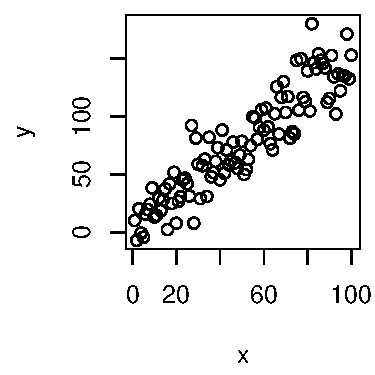
\includegraphics[bb=0in 0in 2.5in 2.5in, height=2.5in, width=2.5in]{Figures/Figure1.pdf}
    \label{fig:FigureAppendix}
\end{figure}

\section{Appendix Title B (EXAMPLE)}
\label{app:AppendixLableB}

These appendices are only here so that I don't loose the template and forget how to insert and reference them in \LaTeX.

The detailed results are shown in Table~\ref{tab:DeckedTable}. 

\begin{table}
  \begin{threeparttable}
    \caption{A More Complex Decked Table}
    \label{tab:DeckedTable}
    \begin{tabular}{@{}lrrr@{}}         \toprule
    Distribution type  & \multicolumn{2}{l}{Percentage of} & Total number   \\
                       & \multicolumn{2}{l}{targets with}  & of trials per  \\
                       & \multicolumn{2}{l}{segment in}    & participant    \\ \cmidrule(r){2-3}
                                    &  Onset  &  Coda            &          \\ \midrule
    Categorical -- onset\tabfnm{a}  &    100  &     0            &  196     \\
    Probabilistic                   &     80  &    20\tabfnm{*}  &  200     \\
    Categorical -- coda\tabfnm{b}   &      0  &   100\tabfnm{*}  &  196     \\ \midrule
    \end{tabular}
    \begin{tablenotes}[para,flushleft]
        {\small
            \textit{Note.} All data are approximate.

            \tabfnt{a}Categorical may be onset.
            \tabfnt{b}Categorical may also be coda.

            \tabfnt{*}\textit{p} < .05.
            \tabfnt{**}\textit{p} < .01.
         }
    \end{tablenotes}
  \end{threeparttable}
\end{table}


\end{document}

%% 
%% Copyright (C) 2019 by Daniel A. Weiss <daniel.weiss.led at gmail.com>
%% 
%% This work may be distributed and/or modified under the
%% conditions of the LaTeX Project Public License (LPPL), either
%% version 1.3c of this license or (at your option) any later
%% version.  The latest version of this license is in the file:
%% 
%% http://www.latex-project.org/lppl.txt
%% 
%% Users may freely modify these files without permission, as long as the
%% copyright line and this statement are maintained intact.
%% 
%% This work is not endorsed by, affiliated with, or probably even known
%% by, the American Psychological Association.
%% 
%% This work is "maintained" (as per LPPL maintenance status) by
%% Daniel A. Weiss.
%% 
%% This work consists of the file  apa7.dtx
%% and the derived files           apa7.ins,
%%                                 apa7.cls,
%%                                 apa7.pdf,
%%                                 README,
%%                                 APA7american.txt,
%%                                 APA7british.txt,
%%                                 APA7dutch.txt,
%%                                 APA7english.txt,
%%                                 APA7german.txt,
%%                                 APA7ngerman.txt,
%%                                 APA7greek.txt,
%%                                 APA7czech.txt,
%%                                 APA7turkish.txt,
%%                                 APA7endfloat.cfg,
%%                                 Figure1.pdf,
%%                                 shortsample.tex,
%%                                 longsample.tex, and
%%                                 bibliography.bib.
%% 
%%
%% End of file `./samples/longsample.tex'.
